%slide di introduzione ai fondamenti degli schemi xml
% Only TYPED xml can be validated with an XML schema
% When XML documents need to follow a certain structure and the values of attributes and elements need to follow a set of rules
% A method to describe the XML structure 
% A method to validate the XML data
%  get a clear idea about the required XML structure from the schema.
% Since a schema explains the required XML structure much better than a word document or a document of any other kind, there are no chances of misunderstanding or misinterpreting what is required.
% Validation of the XML data submitted by the client applications became easier.
%  define the validation rules.
%  list of validations that had to be included in the Schema



% frame 02
\begin{frame}
    \frametitle{Elementi per la definizione degli schemi xml}
    \framesubtitle{principi}
    \addtocounter{nframe}{1}

    we need to make sure that the data that we receive follows a certain XML structure and should contain values which are coherent. 

    Your function needs to make sure that the caller passes correct XML data. You could make use of an XML Schema to perform this validation.

    Performing such validations without the help of a SCHEMA will be extremely difficult most of the time.


\end{frame}

% frame 03
\begin{frame}
    \frametitle{Elementi per la definizione degli schemi xml}
    \framesubtitle{principi}
    \addtocounter{nframe}{1}

    Make sure that the XML document is structured exactly the way your function expects it to be.

   We need an XML schema when we need to make sure that the XML document that we need to work with is in the expected format.
   Make sure that the values of elements and attributes are within the accepted range.

   When data is managed and exchanged in XML format, there needs to be clear agreement about the structure of the XML document.

   There needs to be a contract between the caller and the callee about the XML document being exchanged.

   validate the XML document to make sure that it adheres to the format defined in the contract.


\end{frame}



% frame 04
\begin{frame}
    \frametitle{Elementi per la definizione degli schemi xml}
    \framesubtitle{principi}
    \addtocounter{nframe}{1}

    A Schema provides such the contract. 
    \\ It defines the structure of the XML document. 
    \\ It defines rules to validate the value of elements and attributes as well as their formats. 
    \\ Once a schema is defined, a Schema Validator can validate an XML document against the rules defined in the Schema.


\end{frame}


% frame 05
\begin{frame}
    \frametitle{Elementi per la definizione degli schemi xml}
    \framesubtitle{Tipi di formalismi per definire schemi XML}
    \addtocounter{nframe}{1}

   DTD, XDR, SOX, Schematron, DSD, DCD, DDML, RELAX NG

\end{frame}

\subsection{DTD}
%slide di introduzione ai fondamenti di Document Type Definition

%frame 01
\begin{frame}
    \frametitle{Elementi per la definizione degli schemi xml}
    \framesubtitle{principi}
    \addtocounter{nframe}{1}

    \begin{block}{Esempio DTD}
        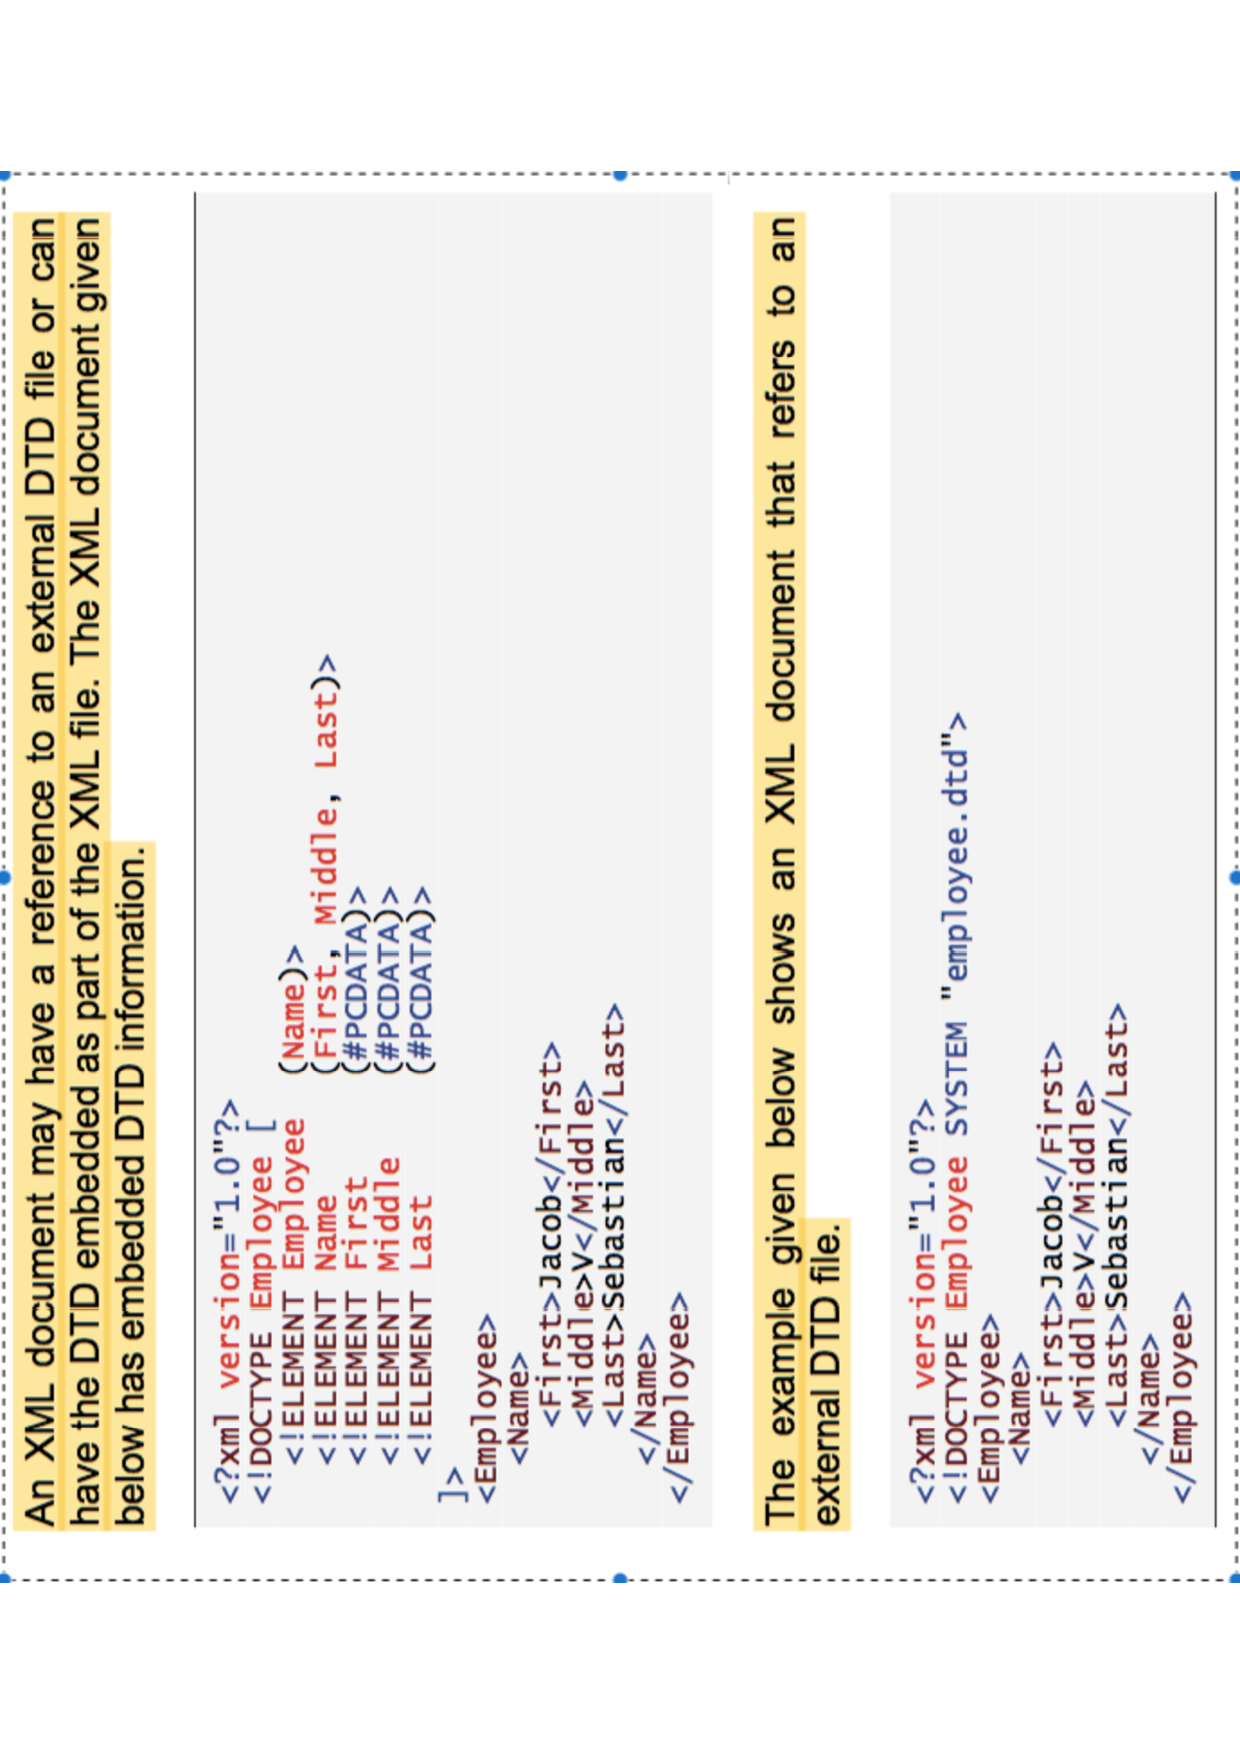
\includegraphics[width=.5\textwidth]{../imgs/dtd_1.pdf}
    \end{block}

\end{frame}

\subsection{XSD}
%slide relative ad introdurre gli elementi di XML Schema Definition (XSD) 

% building blocks of an XSD Schema at the most granular level are elements and attributes
% bigger blocks are built using basic components: elements and attributes.
% declaring elements and attributes, adding child elements, defining occurrence and order of child elements
% XSD data types and see how to perform basic data validation using XSD.

% Writing the XSD code for describing and validating an element in an XML document is called element declaration.

%% Element declaration
% The element declaration we created above has an attribute named name.
% This attribute specifies the name of the element expected in the XML instance document
% esistono altri attributi dell'elemento xsd per la dichiarazione di elementi

%% Attribute declaration
% The XSD code to describe and validate an attribute in an XML instance document is called attribute declaration.
% An attribute cannot exist without a parent element;

%% Esempio element declaration più attribute declaration
%  <xsd:schema xmlns:xsd="http://www.w3.org/2001/XMLSchema">
%   <xsd:element name="Employee">
%     <xsd:complexType>
%       <xsd:attribute name="Name"/>
%     </xsd:complexType>
%   </xsd:element>
% </xsd:schema>

%% Element Types
% An element may have a simple type or complex type based on its structure/content.
% It has a simple type if it does not have any child element or attribute 
% If it has an attribute or contains other child elements, it has a complex type.


%% Simple Types
Elements that do not have child elements or attributes are simple type elements.
%% Complex Type


%frame 01
\begin{frame}
    \frametitle{Elementi per la definizione degli schemi xml}
    \framesubtitle{principi}
    \addtocounter{nframe}{1}

    \begin{block}{Cos'è uno schema XML}
     
    Uno schema XSD è un document XML standard.

    An XML Schema is a document which describes another XML document. 
    \\ XML Schemas are used to validate XML documents. 
    \\ An XML schema itself is an XML document which contains the rules to be validated against a given XML instance document
    \end{block}

\end{frame}

%frame 02
\begin{frame}
    \frametitle{Elementi per la definizione degli schemi xml}
    \framesubtitle{principi XSD}
    \addtocounter{nframe}{1}

    \begin{block}{XSD esempio}
        Grazie agli schemi XSD è possibile definire tutte gli elementi e le regole per la corretta strutturazione e la validazione di un documento XML.
    \end{block}

    \begin{block}{XSD Schema}
        Il termine XSD o XML schema si riferisce ad un documento XML che descrive e valida la struttura e il contenuto di un altro documento XML.
        (dichiarazione del documento (declaration) e istanza del documento (instance))
    \end{block}
    
\end{frame}


%frame 03
\begin{frame}
    \frametitle{Elementi per la definizione degli schemi xml}
    \framesubtitle{principi XSD}
    \addtocounter{nframe}{1}

    \begin{block}{XSD esempio}
         The root element of an XML schema should always be the "<schema>" element. All definitions should appear under the root element "<schema>."
    \end{block}

    \begin{block}{XSD Schema}
        All elements and attributes of XML Schema are declared in the namespace "http://www.w3.org/2001/XMLSchema." Hence, every XML schema document should contain the above namespace declaration.
    \end{block}
    
\end{frame}


%frame 04
\begin{frame}
    \frametitle{Elementi per la definizione degli schemi xml}
    \framesubtitle{principi XSD}
    \addtocounter{nframe}{1}

    \defverbatim{\xsdfirst}{%
    \begin{tiny}
    \begin{verbatim}
        <xsd:schema xmlns:xsd="http://www.w3.org/2001/XMLSchema">
            <xsd:element name="text"/>
        </xsd:schema>
    \end{verbatim}
    \end{tiny}
    }

     \defverbatim{\xmlfirst}{%
    \begin{tiny}
    \begin{verbatim}
             <text>Il primo documento XML Validato</text>
    \end{verbatim}
    \end{tiny}
    }


    \begin{block}{XSD esempio}
        {\xsdfirst}
    \end{block}

    \begin{block}{XML XSD esempio}
        
        The XML Instance Document of this schema should contain a root element named text. Here is a valid XML instance document which successfully validates against this schema.
        {\xmlfirst}

    \end{block}
    
\end{frame}


% slide 05 perform validation
%   xmllint xmlfirst.xml --schema ../schema/xsd/xsdfirst.xsd


\subsection{RELAXGN}
\input{relaxng.tex}